\documentclass[notes,11pt, aspectratio=169, xcolor=table]{beamer}

\usepackage{pgfpages}
% These slides also contain speaker notes. You can print just the slides,
% just the notes, or both, depending on the setting below. Comment out the want
% you want.
\setbeameroption{hide notes} % Only slide
%\setbeameroption{show only notes} % Only notes
%\setbeameroption{show notes on second screen=right} % Both

\usepackage{helvet}
\usepackage[default]{lato}
\usepackage{array}

\newtheorem{proposition}{Proposition}

\usepackage{tikz}
\usetikzlibrary{shapes.geometric}
\usepackage{pgfplots}
\usepackage{graphicx}
\usepackage{verbatim}
\setbeamertemplate{note page}{\pagecolor{yellow!5}\insertnote}
\usetikzlibrary{positioning}
\usetikzlibrary{snakes}
\usetikzlibrary{calc}
\usetikzlibrary{arrows}
\usetikzlibrary{decorations.markings}
\usetikzlibrary{shapes.misc}
\usetikzlibrary{matrix,shapes,arrows,fit,tikzmark}
\usepackage{amsmath}
\usepackage{mathpazo}
\usepackage{hyperref}
\usepackage{lipsum}
\usepackage{multimedia}
\usepackage{graphicx}
\usepackage{multirow}
\usepackage{graphicx}
\usepackage{dcolumn}
\usepackage{bbm}
\usepackage[style=authoryear,sorting=nyt,uniquename=false]{biblatex}
\newcommand{\blue}[1]{\textcolor{blue}{#1}}
\newcommand{\white}[1]{\textcolor{white}{#1}}

\addbibresource{references.bib} 

\newcolumntype{d}[0]{D{.}{.}{5}}

\def\@@mybluebox[#1][#2]#3{
    \sbox\mytempbox{#3}%
    \mytemplen\ht\mytempbox
    \advance\mytemplen #1\relax
    \ht\mytempbox\mytemplen
    \mytemplen\dp\mytempbox
    \advance\mytemplen #2\relax
    \dp\mytempbox\mytemplen
    \colorbox{myblue}{\hspace{1em}\usebox{\mytempbox}\hspace{1em}}}


\usepackage{changepage}
\usepackage{appendixnumberbeamer}
\newcommand{\beginbackup}{
   \newcounter{framenumbervorappendix}
   \setcounter{framenumbervorappendix}{\value{framenumber}}
   \setbeamertemplate{footline}
   {
     \leavevmode%
     \hline
     box{%
       \begin{beamercolorbox}[wd=\paperwidth,ht=2.25ex,dp=1ex,right]{footlinecolor}%
%         \insertframenumber  \hspace*{2ex} 
       \end{beamercolorbox}}%
     \vskip0pt%
   }
 }
\newcommand{\backupend}{
   \addtocounter{framenumbervorappendix}{-\value{framenumber}}
   \addtocounter{framenumber}{\value{framenumbervorappendix}} 
}


\usepackage{graphicx}
\usepackage[space]{grffile}
\usepackage{booktabs}

% These are my colors -- there are many like them, but these ones are mine.
\definecolor{blue}{RGB}{0,114,178}
\definecolor{red}{RGB}{213,94,0}
\definecolor{yellow}{RGB}{240,228,66}
\definecolor{green}{RGB}{0,158,115}

\hypersetup{
  colorlinks=false,
  linkbordercolor = {white},
  linkcolor = {blue}
}


%% I use a beige off white for my background
\definecolor{MyBackground}{RGB}{255,253,218}

%% Uncomment this if you want to change the background color to something else
%\setbeamercolor{background canvas}{bg=MyBackground}

%% Change the bg color to adjust your transition slide background color!
\newenvironment{transitionframe}{
  \setbeamercolor{background canvas}{bg=yellow}
  \begin{frame}}{
    \end{frame}
}

\setbeamercolor{frametitle}{fg=blue}
\setbeamercolor{title}{fg=blue}
\setbeamertemplate{footline}[frame number]
\setbeamertemplate{navigation symbols}{} 
\setbeamertemplate{itemize items}{-}
\setbeamercolor{itemize item}{fg=blue}
\setbeamercolor{itemize subitem}{fg=blue}
\setbeamercolor{enumerate item}{fg=blue}
\setbeamercolor{enumerate subitem}{fg=blue}
\setbeamercolor{button}{bg=MyBackground,fg=blue,}



% If you like road maps, rather than having clutter at the top, have a roadmap show up at the end of each section 
% (and after your introduction)
% Uncomment this is if you want the roadmap!
% \AtBeginSection[]
% {
%    \begin{frame}
%        \frametitle{Roadmap of Talk}
%        \tableofcontents[currentsection]
%    \end{frame}
% }
\setbeamercolor{section in toc}{fg=blue}
\setbeamercolor{subsection in toc}{fg=red}
\setbeamersize{text margin left=1em,text margin right=1em} 

\newenvironment{wideitemize}{\itemize\addtolength{\itemsep}{10pt}}{\enditemize}

\usepackage{environ}
\NewEnviron{videoframe}[1]{
  \begin{frame}
    \vspace{-8pt}
    \begin{columns}[onlytextwidth, T] % align columns
      \begin{column}{.58\textwidth}
        \begin{minipage}[t][\textheight][t]
          {\dimexpr\textwidth}
          \vspace{8pt}
          \hspace{4pt} {\Large \sc \textcolor{blue}{#1}}
          \vspace{8pt}
          
          \BODY
        \end{minipage}
      \end{column}%
      \hfill%
      \begin{column}{.42\textwidth}
        \colorbox{green!20}{\begin{minipage}[t][1.2\textheight][t]
            {\dimexpr\textwidth}
            Face goes here
          \end{minipage}}
      \end{column}%
    \end{columns}
  \end{frame}
}

\title[]{International Trade: Lecture 1}
\subtitle[]{The Principle of Comparative Advantage}
\author[Góes]
{Carlos Góes\inst{1}}
\date{Fall 2025}
\institute[GWU]{\inst{1} George Washington University }



\begin{document}

%%% TIKZ STUFF
\tikzset{   
        every picture/.style={remember picture,baseline},
        every node/.style={anchor=base,align=center,outer sep=1.5pt},
        every path/.style={thick},
        }
\newcommand\marktopleft[1]{%
    \tikz[overlay,remember picture] 
        \node (marker-#1-a) at (-.3em,.3em) {};%
}
\newcommand\markbottomright[2]{%
    \tikz[overlay,remember picture] 
        \node (marker-#1-b) at (0em,0em) {};%
}
\tikzstyle{every picture}+=[remember picture] 
\tikzstyle{mybox} =[draw=black, very thick, rectangle, inner sep=10pt, inner ysep=20pt]
\tikzstyle{fancytitle} =[draw=black,fill=red, text=white]
%%%% END TIKZ STUFF



%----------------------------------------------------------------------%
%-------------------       TITLE PAGE       ---------------------------%
%----------------------------------------------------------------------%





%----------------------------------------------------------------------%






%----------------------------------------------------------------------%
%----------------------------------------------------------------------%

%----------------------------------------------------------------------%
\frame{\titlepage}
\addtocounter{framenumber}{-1}
%----------------------------------------------------------------------%



%----------------------------------------------------------------------%
%----------------------------------------------------------------------%

\begin{frame}{Motivation}

\begin{wideitemize}
    \item Economists (and scientists in general) work with \blue{models}
    \item<2-> Why?
    \item<2-> What do you think the purpose of models is?
    \item<3-> Sometimes people criticize models for being ``unrealistic''
    \item<4-> When this a reasonable criticism?
    \item<5-> \blue{My claim}: a good model \textit{must} simplify reality
\end{wideitemize}
    
\end{frame}



 \begin{frame}{What science truly means}
  \makebox[\linewidth][c]{
    \resizebox{0.8\linewidth}{!}{
    
\includegraphics{figs/borges.PNG}
      }
    }
\end{frame}

 \begin{frame}{Most beautiful intro in all of economics}
  \makebox[\linewidth][c]{
    \resizebox{0.8\linewidth}{!}{
    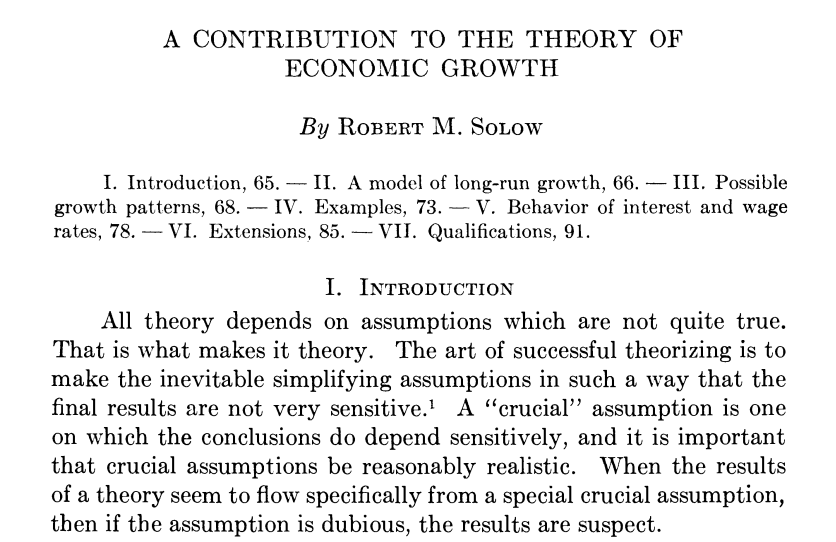
\includegraphics{figs/solow-all-theory.PNG}
      }
    }
    
    \end{frame}

\begin{frame}{Initial takeaway}

\begin{wideitemize}
    \item \blue{My claim}: a good model \textit{must} simplify reality
    \item<2-> A theory that tries to model everything is a bad theory
    \item<3-> Why? It obfuscates rather than illuminates.
    \item<4-> The point of science is to explain some causal relationship.
    \item<5-> Solow: crucial assumptions to explain that causal relationship must be  realistic.
\end{wideitemize}
    
\end{frame}


\section{How to think like an economist}

\begin{frame}{How to think like a economist  (or like most scientists)?}
 \begin{wideitemize}
    \item Document the facts
    \item Develop a simplified a model
    \item Compare the predictions of the model with the original facts (i.e., test the model)
    \item Use the model to make other predictions that may eventually be tested (i.e., run counterfactual experiments with the model).
 \end{wideitemize}
\end{frame}


\begin{frame}{What is a model?}
  \makebox[\linewidth][c]{
    \resizebox{0.8\linewidth}{!}{
    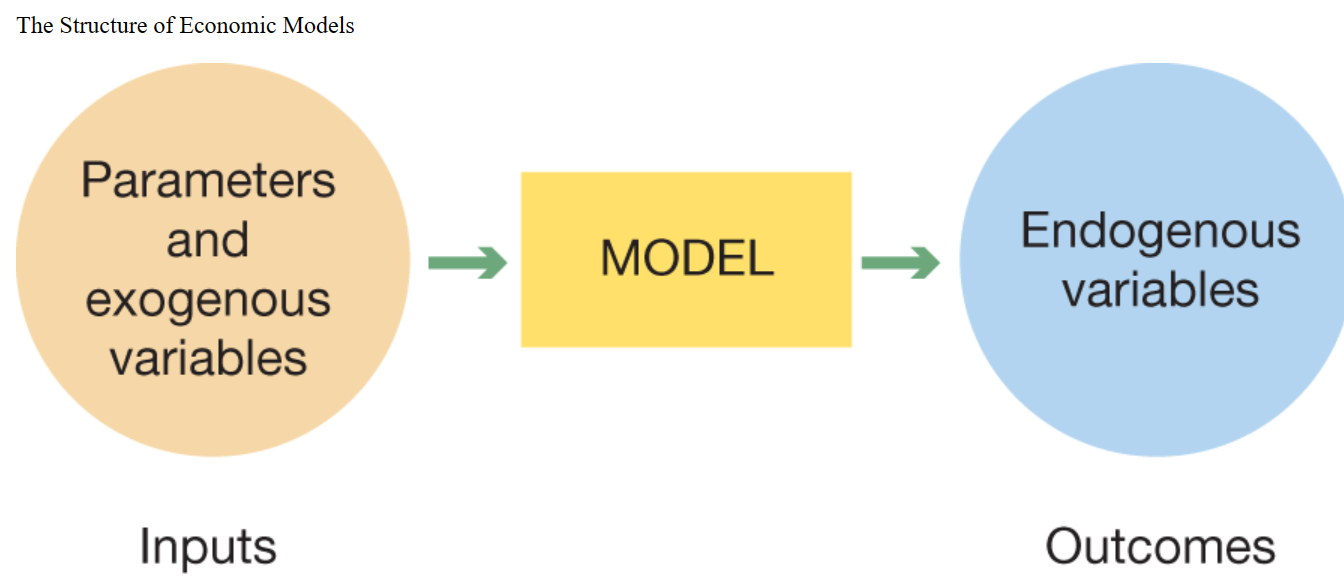
\includegraphics{figs/models.PNG}
      }
    }\end{frame}

\begin{frame}{A model in HS physics}
  \makebox[\linewidth][c]{
    \resizebox{0.8\linewidth}{!}{
    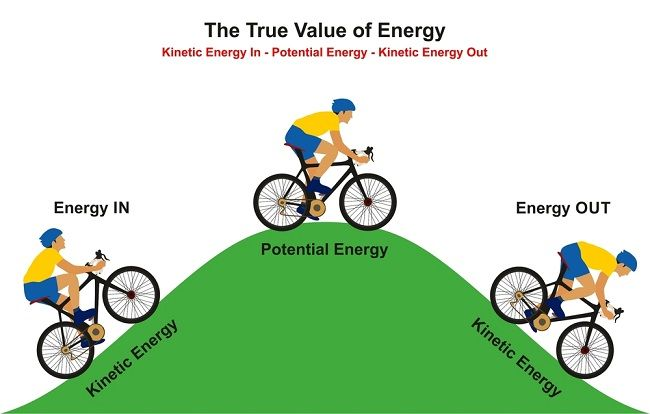
\includegraphics{figs/model-in-physics.jpg}
      }
    }
    
    \end{frame}

\begin{frame}{A model in Econ 101}
  \makebox[\linewidth][c]{
    \resizebox{0.55\linewidth}{!}{
    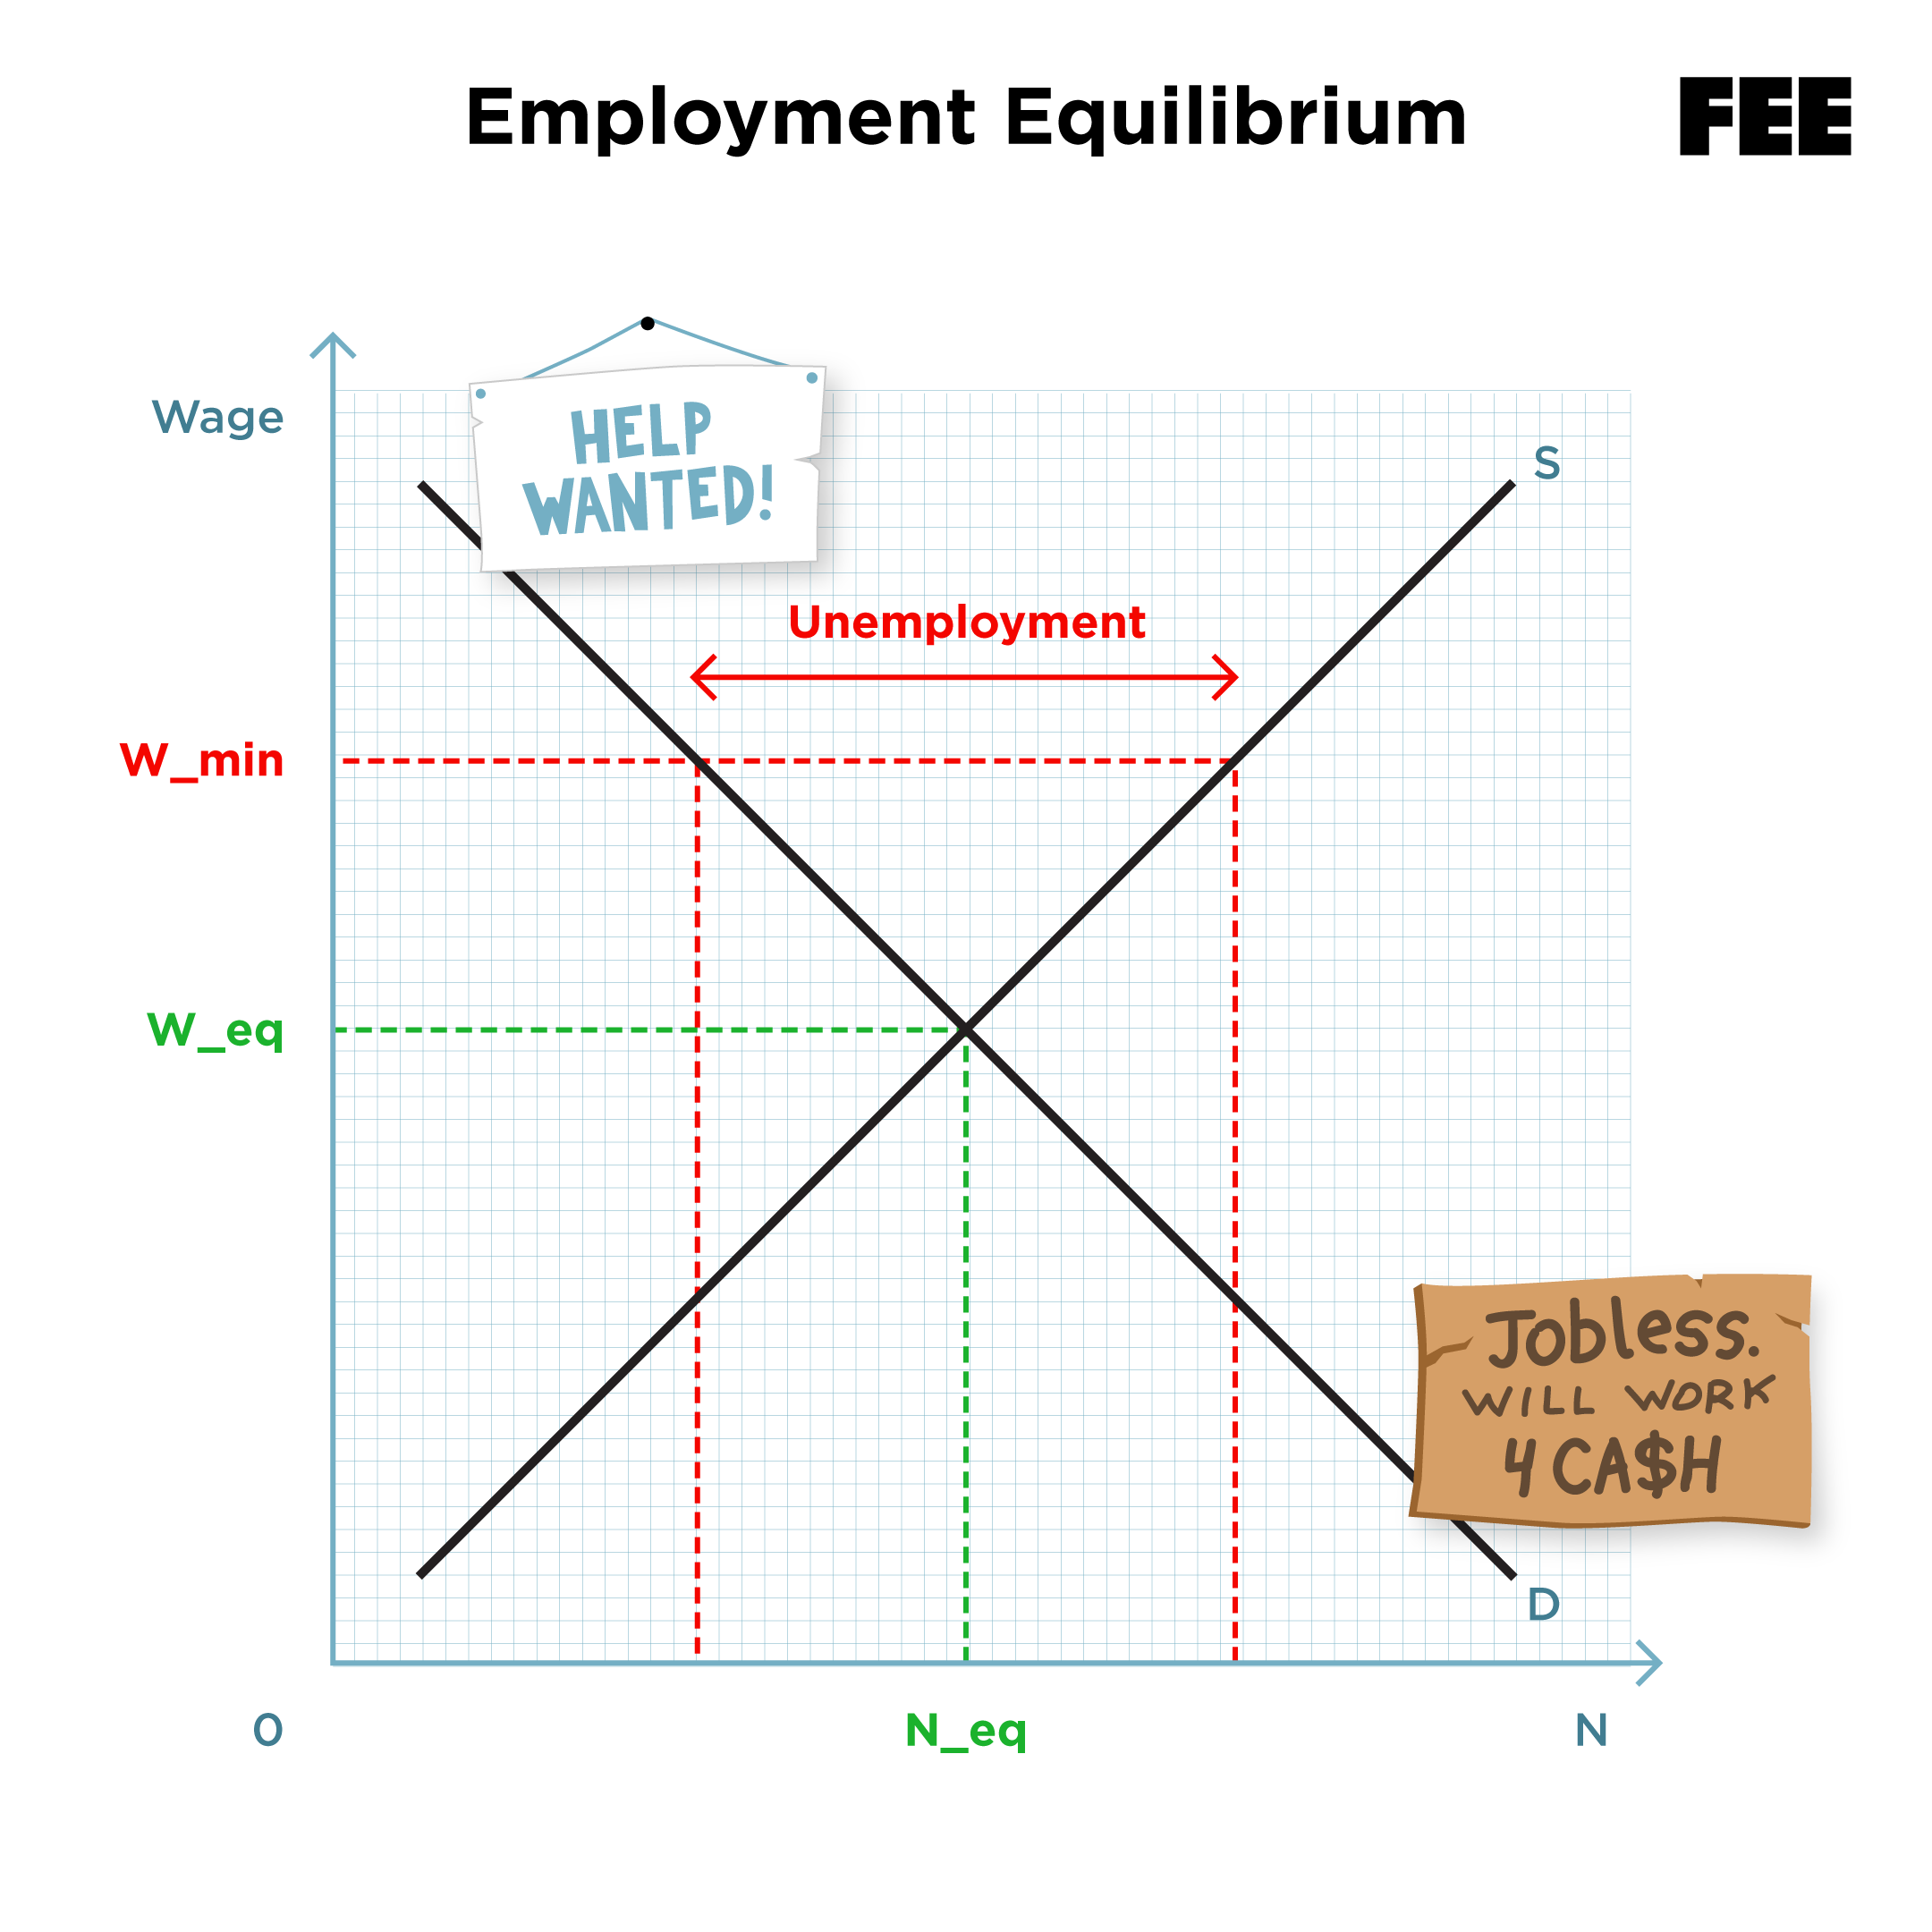
\includegraphics{figs/employment-equilibrium.png}
      }
    }\end{frame}


\begin{frame}{Questions: can the model explain reality?}
 \begin{wideitemize}
    \item If so, in what circumstances?
    \item If not why? 
    \item<2-> In the real world, neither model fully generalizes.
    \item<3-> It depends on the particular context: friction, air resistance, temperature; pressure... economic frictions, market power, government policy, migration, international trade, etc...
    \item<4-> But they both can   explain the world \textit{under certain assumptions}...
 \end{wideitemize}
\end{frame}

 \begin{frame}{Two models in Econ 201}
 \begin{figure}
    \centering
    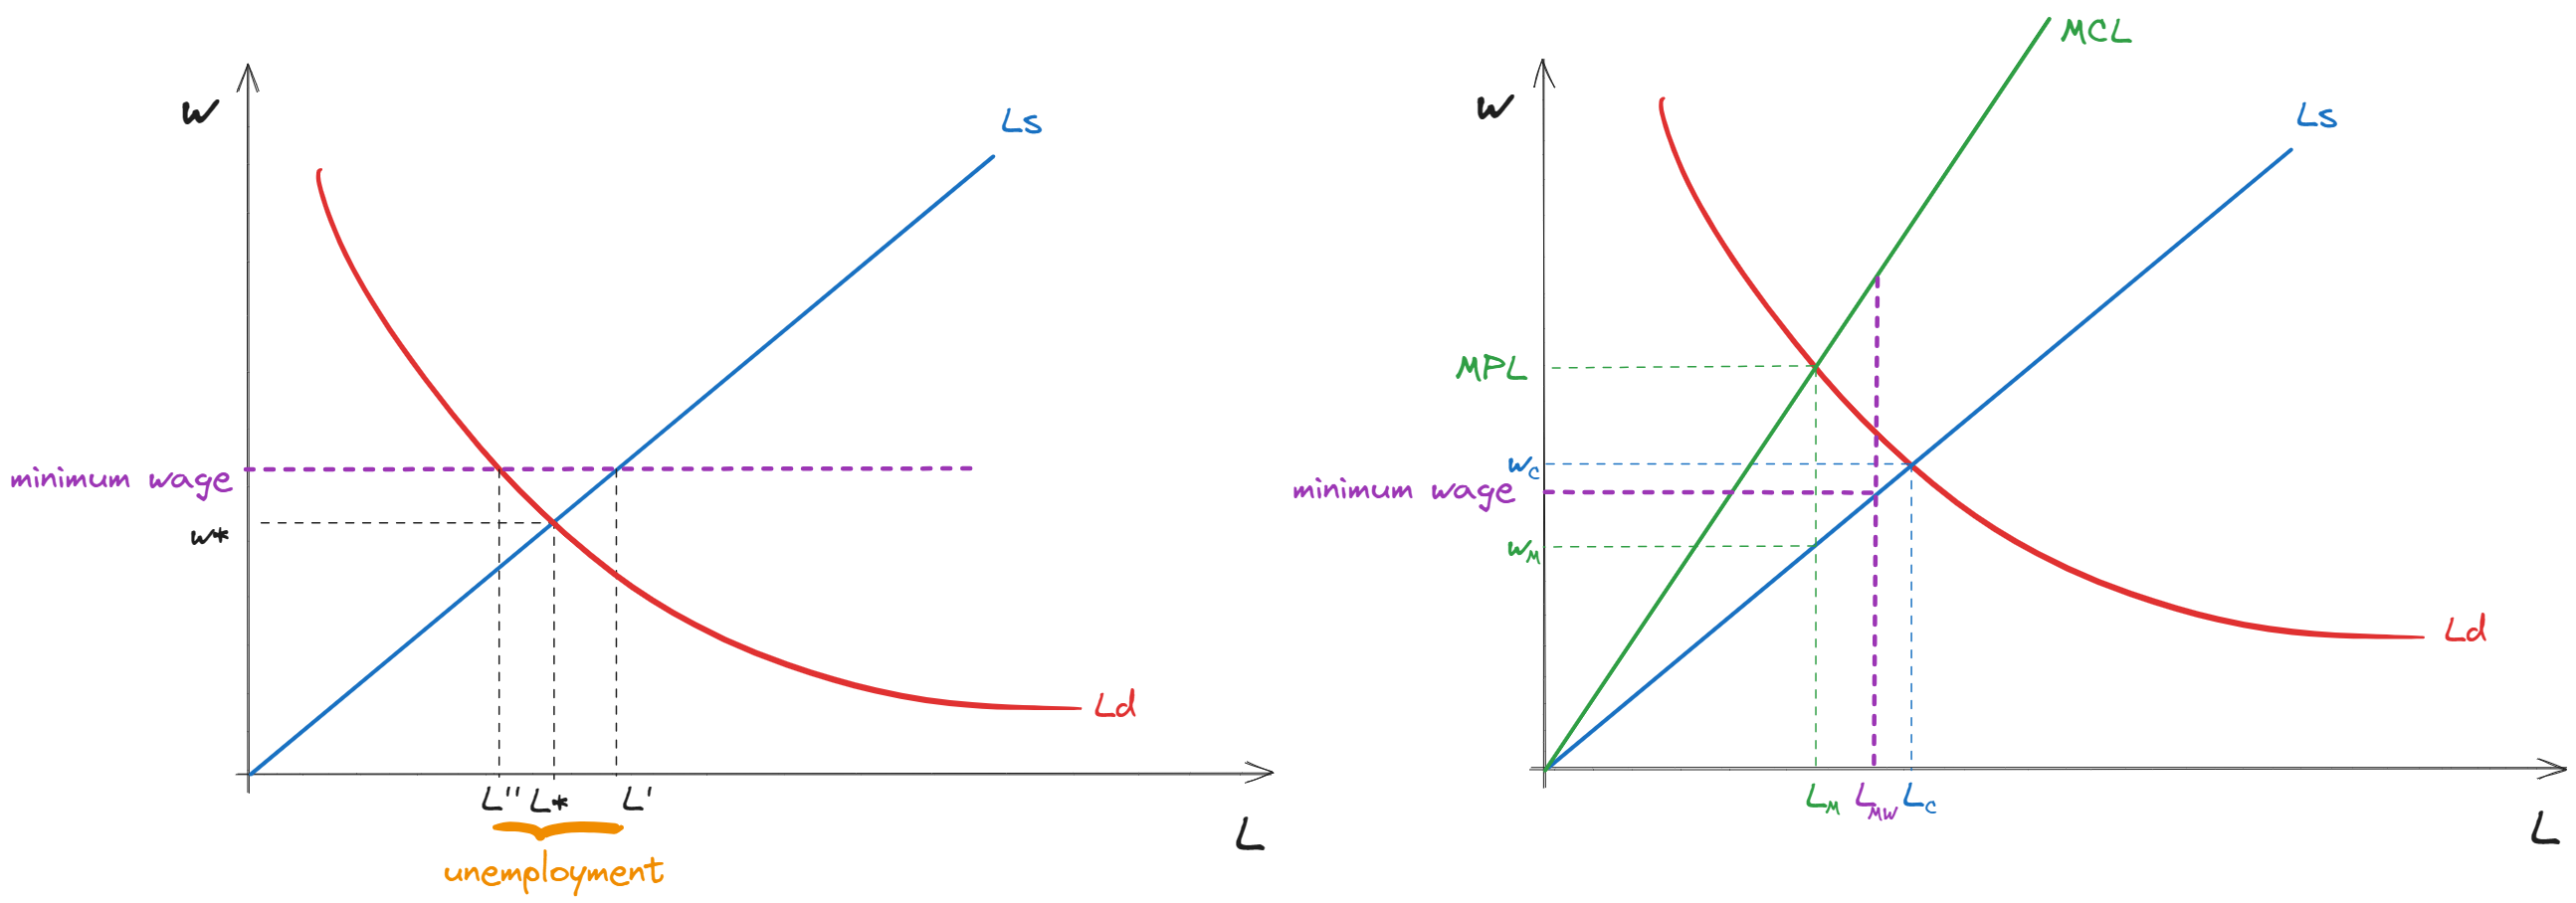
\includegraphics[width=\textwidth]{figs/mw-competitive-monopsony.png}
\end{figure}
 \end{frame}

  \begin{frame}{The Minimum Wage and Labor Market Structure}

  \begin{wideitemize}
  \item Under perfectly competitive labor market, the minimum wage results in
lower labor demand, and unemployment
    \item  Under monopsony, the minimum wages results in higher labor supply, and lower unemployment
    \item \textbf{Bottom Line}: the stylized labor market we have studied should be used with extra care when thinking about labor market policies!
    \item \textbf{But context matters}: \textcolor{blue}{even under monopsony, there are limits to the minimum wage}!
  \end{wideitemize}

  \end{frame}

\begin{frame}{What is a counterfactual experiment?}
 \begin{wideitemize}
    \item What happens if we change a parameter in the model?
    \item<2-> Gravity, temperature, altitude...?
    \item<3-> Taxes, government expenditure, inflation, elasticities, etc...?
    \item<4-> How would our predictions change? How does that align with reality? Which of these parameters can we observe? Which of them do we have to calibrate indirectly?
 \end{wideitemize}
\end{frame}

\section{Intro}

\begin{frame}{Why do we trade?}
\begin{wideitemize}
    \item Have you engaged in trade today?
\onslide<3->{
    \begin{itemize}
        \item You all are trading your future (hopefully higher) income for my teaching;
        \item I am teaching so that I can pay for my wife's handbags;
    \end{itemize}
}
\onslide<3->{
    \item What makes countries (or people) trade?
}
\onslide<4->{
    \vspace{12pt}

    \begin{itemize}
        \item Different skills (e.g., I am bad mechanic, so I pay Jiffy Lube instead)
        \item Different endowments (e.g., Saudi Arabia has a lot of oil; Luxembourg does not);
        \item Different products (e.g., both France and Italy produce wine, but trade for variety);
    \end{itemize}
}
\end{wideitemize}    
\end{frame}

\begin{frame}{Why do we trade?}
\begin{wideitemize}
    \item Is trade \textcolor{blue}{\textbf{desirable}?} 
    \vspace{12pt}

    \begin{quote}
        ``We don’t win on trade. You will find out that we have an unbelievably bad trade deficit with every country.'' ~ \href{https://www.c-span.org/program/public-affairs-event/donald-trump-remarks/244635}{Donald Trump, CPAC 2011}
    \end{quote}
\onslide<2>{
    \item Should we try to produce most things at home? 
    \vspace{12pt}

    \begin{quote}
        ``To preserve the ballance of trade in favour of a nation ought to be a leading aim of its policy. The avarice of individuals may frequently find its account in pursuing channels of traffic prejudicial to that ballance, to which the government may be able to oppose effectual impediments.'' ~ \href{https://founders.archives.gov/documents/Hamilton/01-03-02-0015}{Alexander Hamilton, The Continentalist V, 1782}
    \end{quote}
}
\end{wideitemize}    
\end{frame}

\begin{frame}{Why do we trade?}
\begin{wideitemize}
    \item Suppose it were true that a country is better off by producing everything at home
\onslide<2->{
\item If it were true across countries, why would it not be true across states?
    \item Should Virginia try to produce oranges rather than importing it from Florida?
}
\onslide<3->{
    \item If it were true across states, why would it not be true across households?    
    \item Should John try to grow his vegetables rather than trading with Whole Foods?
    \item ... and try to sewn his own clothes rather than trading with Macy's?
}
\onslide<4->{
    \item Would they be better off? 
}
\end{wideitemize}    
\end{frame}

\begin{frame}{Why do we trade?}
\begin{wideitemize}
    \item In short, we trade because \textcolor{blue}{trade makes us richer}, i.e. able to consume more.
\onslide<2->{
    \item If I try to own my own clothes, I will end up with bad clothes and waste time I could be exchanging for dollars.

    \item I am better off specializing in being an economist... and trading.
}
\onslide<3->{
\vspace{12pt}
        
    \begin{quote}
        ``It is the maxim of every prudent master of a family, never to attempt to make at home what it will cost him more to make than to buy. […] What is prudence in the conduct of every private family, can scarce be folly in that of a great kingdom.'' ~ \href{https://www.econlib.org/library/Smith/smWN.html?chapter_num=27#book-reader}{Adam Smith, The Wealth of Nations, 1776}
    \end{quote}
}
\end{wideitemize}
    
\end{frame}

\section{The principle of comparative advantage}

\begin{frame}{The principle of comparative advantage}
    \begin{wideitemize} 
        \item What we described above is the \textcolor{blue}{principle of comparative advantage}
\onslide<2->{
        \item Countries/households will be better off by specializing in subset of activities + trading
}
    \end{wideitemize}
\vspace{24pt}
\onslide<3->{
        \Huge
        \centering
        we call these \textcolor{blue}{gains from trade}
        \normalsize
}
\end{frame}

\begin{frame}{The principle of comparative advantage}
    \begin{wideitemize} 
        \item Consider a world with 2 countries (US, Colombia) and 2 products (computers, roses)
        \item<2-> Colombia can produce 9 million roses or 10,000 computers
        \begin{itemize}
            \item Opportunity cost: $1/900$ computers per rose
        \end{itemize}
        \item<3-> US can produce 10 million roses or 100,000 computers
        \begin{itemize}
            \item Opportunity cost: $1/100$ computers per rose
        \end{itemize}
        \item<4-> Note the US can produce more computers and more roses!
        \item<5-> Can trade make US workers (as an aggregate) better off?
    \end{wideitemize}
\end{frame}



\begin{frame}{Production Possibilities Frontier: Numerical Example}
\begin{center}
\begin{tabular}{@{} l >{\centering\arraybackslash}m{0.35\linewidth} >{\centering\arraybackslash}m{0.35\linewidth} @{}}
\toprule
& \textbf{US} & \textbf{Colombia} \\
\midrule
\textbf{Opportunity cost} 
& $\dfrac{1}{100}$ \textbf{computers} \newline \textbf{per rose}
& $\dfrac{1}{900}$ \textbf{computers} \newline \textbf{per rose} \\
\addlinespace[1ex]
\textbf{Autarky consumption} 
& 10 million \textbf{roses} \newline 100,000 \textbf{computers} 
& 9 million \textbf{roses} \newline 10,000 \textbf{computers}   \\
\addlinespace[1ex]
\bottomrule
\end{tabular}

\vspace{1em}
\textit{All output measured in terms of roses for comparison}


\end{center}
\end{frame}

\begin{frame}{Production Possibilities Frontier in Autarky}
\begin{center}

\begin{figure}[htbp]

% US
\begin{subfigure}{}
\resizebox{0.48\linewidth}{!}{%
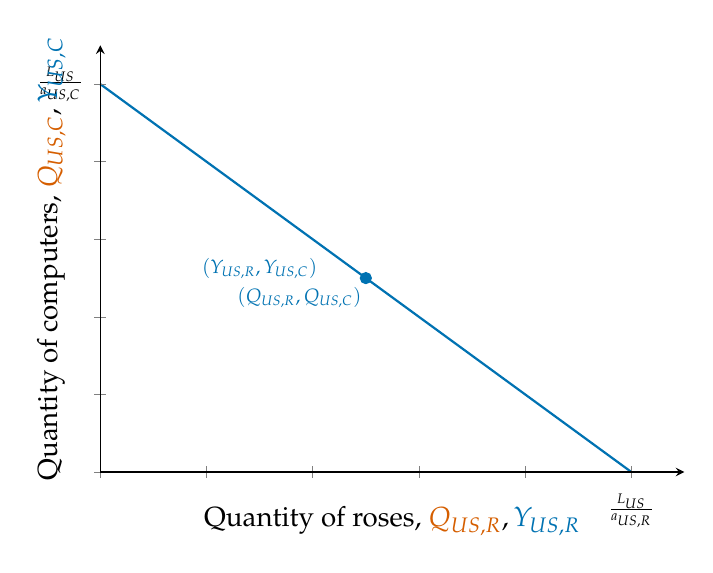
\begin{tikzpicture}
\pgfmathsetmacro{\aC}{100}       % unit labor requirement for computers
\pgfmathsetmacro{\aR}{1}         % unit labor requirement for roses
\pgfmathsetmacro{\alpha}{0.5}    % preference for computers
\pgfmathsetmacro{\Lendow}{10}    % labor endowment

% Compute equilibrium quantities
\pgfmathsetmacro{\Qc}{(\alpha*\Lendow)/\aC}
\pgfmathsetmacro{\Qr}{((1 - \alpha)*\Lendow)/\aR}

% Compute utility level
\pgfmathsetmacro{\U}{(\Qc^(\alpha))*(\Qr^(1 - \alpha))}

% Compute prefactor for indifference curve: Qc = A * Qr^(- (1 - alpha)/alpha)
\pgfmathsetmacro{\expo}{(1 - \alpha)/\alpha}
\pgfmathsetmacro{\A}{\U^(1/\alpha)}

\centering
\begin{axis}[
    ylabel={Quantity of computers, $\textcolor{red}{Q_{US,C}}, \textcolor{blue}{Y_{US,C}}$},
    xlabel={Quantity of roses, $\textcolor{red}{Q_{US,R}}, \textcolor{blue}{Y_{US,R}}$},
    ymin=0, ymax=0.11,
    xmin=0, xmax=11,
    yticklabel=\empty,
    xticklabel=\empty,
    axis lines=left,
    enlargelimits=false,
    clip=false,
    axis on top,
    scaled x ticks=false,
    width=9cm, height=7cm,
    title style={font=\bfseries}
]

% PPF: Q_C = (L/a_C) - (a_R/a_C) * Q_R
\addplot[thick, blue, domain=0:10] {\Lendow/\aC - (\aR/\aC)*x};

% Indifference curve through optimal bundle
%\addplot[red, domain=0.1:9, samples=100] {\A * x^(-\expo)};

% Labels

%\node at (axis cs:3.5,0.03) {\Large $\mathcal{Y}_{US}$};
\node at (axis cs:\Lendow/\aR,-.01) {\scriptsize $\frac{L_{US}}{a_{US,R}}$};
\node at (axis cs:-.75,\Lendow/\aC) {\scriptsize $\frac{L_{US}}{a_{US,C}}$};


% Equilibrium point
\addplot[only marks, mark=*, color=blue, mark size=2pt] coordinates {(\Qr, \Qc)};
\node at (axis cs:\Qr - 1.25,\Qc - 0.005) {\scriptsize $\textcolor{blue}{(Q_{US,R},Q_{US,C})}$};
\node at (axis cs:\Qr - 2,\Qc + 0.0025) {\scriptsize $\textcolor{blue}{(Y_{US,R},Y_{US,C})}$};



\end{axis}

\end{tikzpicture}
}
\end{subfigure}
%
% Colombia
\begin{subfigure}{}
\resizebox{0.48\linewidth}{!}{%
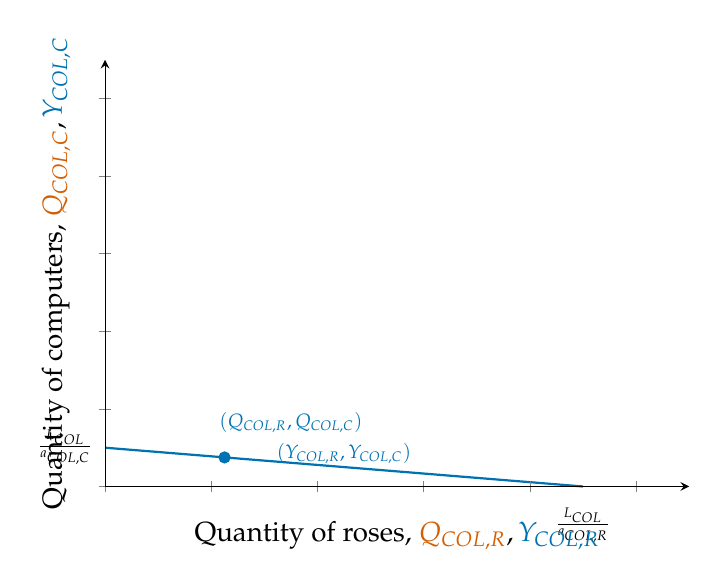
\begin{tikzpicture}
\pgfmathsetmacro{\aC}{900}       % unit labor requirement for computers
\pgfmathsetmacro{\aR}{1}         % unit labor requirement for roses
\pgfmathsetmacro{\alpha}{0.75}    % preference for computers
\pgfmathsetmacro{\Lendow}{9}    % labor endowment

% Compute equilibrium quantities
\pgfmathsetmacro{\Qc}{(\alpha*\Lendow)/\aC}
\pgfmathsetmacro{\Qr}{((1 - \alpha)*\Lendow)/\aR}

% Compute utility level
\pgfmathsetmacro{\U}{(\Qc^(\alpha))*(\Qr^(1 - \alpha))}

% Compute prefactor for indifference curve: Qc = A * Qr^(- (1 - alpha)/alpha)
\pgfmathsetmacro{\expo}{(1 - \alpha)/\alpha}
\pgfmathsetmacro{\A}{\U^(1/\alpha)}

\centering
\begin{axis}[
    ylabel={Quantity of computers, $\textcolor{red}{Q_{COL,C}}, \textcolor{blue}{Y_{COL,C}}$},
    xlabel={Quantity of roses, $\textcolor{red}{Q_{COL,R}}, \textcolor{blue}{Y_{COL,R}}$},
    ymin=0, ymax=0.11,
    xmin=0, xmax=11,
    yticklabel=\empty,
    xticklabel=\empty,
    axis lines=left,
    enlargelimits=false,
    clip=false,
    axis on top,
    scaled x ticks=false,
    width=9cm, height=7cm,
    title style={font=\bfseries}
]

% PPF: Q_C = (L/a_C) - (a_R/a_C) * Q_R
\addplot[thick, blue, domain=0:9] {\Lendow/\aC - (\aR/\aC)*x};

% Indifference curve through optimal bundle
%\addplot[red, domain=0.1:9, samples=100] {\A * x^(-\expo)};

% Labels

%\node at (axis cs:3.5,0.03) {\Large $\mathcal{Y}_{US}$};
\node at (axis cs:\Lendow/\aR,-.01) {\scriptsize $\frac{L_{COL}}{a_{COL,R}}$};
\node at (axis cs:-.75,\Lendow/\aC) {\scriptsize $\frac{L_{COL}}{a_{COL,C}}$};


% Equilibrium point
\addplot[only marks, mark=*, color=blue, mark size=2pt] coordinates {(\Qr, \Qc)};
\node at (axis cs:\Qr + 1.25,\Qc + 0.009) {\scriptsize $\textcolor{blue}{(Q_{COL,R},Q_{COL,C})}$};
\node at (axis cs:\Qr + 2.25,\Qc + 0.001) {\scriptsize $\textcolor{blue}{(Y_{COL,R},Y_{COL,C})}$};


\end{axis}

\end{tikzpicture}
}

\end{subfigure}

\caption{Autarky Equilibrium}
\end{figure}
\end{center}
\end{frame}



\begin{frame}{The principle of comparative advantage}
\begin{center}
\begin{tabular}{@{} l >{\centering\arraybackslash}m{0.35\linewidth} >{\centering\arraybackslash}m{0.35\linewidth} @{}}
\toprule
& \textbf{US} & \textbf{Colombia} \\
\midrule
\textbf{Opportunity cost} 
& $\dfrac{1}{100}$ \textbf{computers} \newline \textbf{per rose}
& $\dfrac{1}{900}$ \textbf{computers} \newline \textbf{per rose} \\
\addlinespace[1ex]
\textbf{Autarky consumption} 
& 10 million \textbf{roses} \newline 100,000 \textbf{computers} 
& 9 million \textbf{roses} \newline 10,000 \textbf{computers}   \\
\addlinespace[1ex]
\textbf{Suppose world price is} 
& \multicolumn{2}{c}{$\dfrac{1}{135}$ \textbf{computers per rose}} \\
\addlinespace[1ex]
\textbf{Specialization} 
& Make 100{,}000 \textbf{computers}; \newline Trade for up to 13.5 million \textbf{roses}
& Grow 9 million \textbf{roses}; \newline Trade for up to 66{,}666 \textbf{computers}  \\
\bottomrule
\end{tabular}

\vspace{1em}
\textit{All output measured in terms of roses for comparison}
\end{center}
\end{frame}


\begin{frame}{Production Possibilities Frontier + Trade Prices}
\begin{center}

\begin{figure}[htbp]

% US
\begin{subfigure}{}
\resizebox{0.48\linewidth}{!}{%
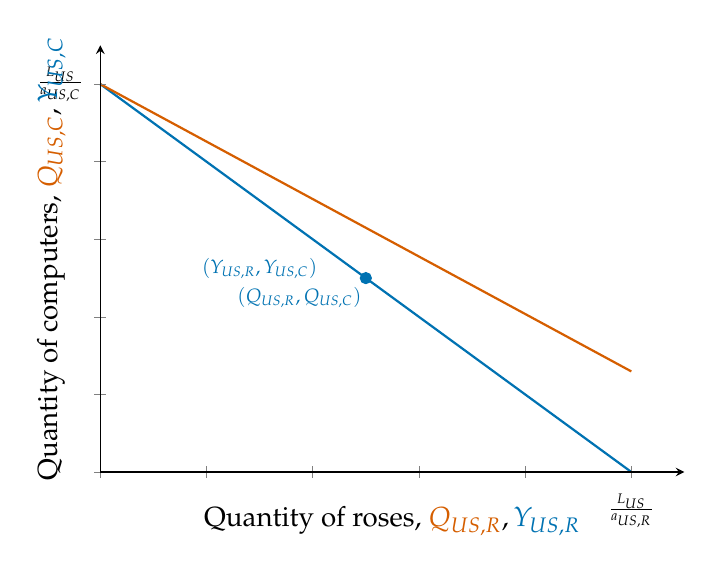
\begin{tikzpicture}
\pgfmathsetmacro{\aC}{100}       % unit labor requirement for computers
\pgfmathsetmacro{\aR}{1}         % unit labor requirement for roses
\pgfmathsetmacro{\alpha}{0.5}    % preference for computers
\pgfmathsetmacro{\Lendow}{10}    % labor endowment

% Compute equilibrium quantities
\pgfmathsetmacro{\Qc}{(\alpha*\Lendow)/\aC}
\pgfmathsetmacro{\Qr}{((1 - \alpha)*\Lendow)/\aR}

% Compute utility level
\pgfmathsetmacro{\U}{(\Qc^(\alpha))*(\Qr^(1 - \alpha))}

% Compute prefactor for indifference curve: Qc = A * Qr^(- (1 - alpha)/alpha)
\pgfmathsetmacro{\expo}{(1 - \alpha)/\alpha}
\pgfmathsetmacro{\A}{\U^(1/\alpha)}

\centering
\begin{axis}[
    ylabel={Quantity of computers, $\textcolor{red}{Q_{US,C}}, \textcolor{blue}{Y_{US,C}}$},
    xlabel={Quantity of roses, $\textcolor{red}{Q_{US,R}}, \textcolor{blue}{Y_{US,R}}$},
    ymin=0, ymax=0.11,
    xmin=0, xmax=11,
    yticklabel=\empty,
    xticklabel=\empty,
    axis lines=left,
    enlargelimits=false,
    clip=false,
    axis on top,
    scaled x ticks=false,
    width=9cm, height=7cm,
    title style={font=\bfseries}
]

% PPF: Q_C = (L/a_C) - (a_R/a_C) * Q_R
\addplot[thick, blue, domain=0:10] {\Lendow/\aC - (\aR/\aC)*x};

\addplot[thick, red, domain=0:10] {\Lendow/\aC - (1/135)*x};


% Indifference curve through optimal bundle
%\addplot[red, domain=0.1:9, samples=100] {\A * x^(-\expo)};

% Labels

%\node at (axis cs:3.5,0.03) {\Large $\mathcal{Y}_{US}$};
\node at (axis cs:\Lendow/\aR,-.01) {\scriptsize $\frac{L_{US}}{a_{US,R}}$};
\node at (axis cs:-.75,\Lendow/\aC) {\scriptsize $\frac{L_{US}}{a_{US,C}}$};


% Equilibrium point
\addplot[only marks, mark=*, color=blue, mark size=2pt] coordinates {(\Qr, \Qc)};
\node at (axis cs:\Qr - 1.25,\Qc - 0.005) {\scriptsize $\textcolor{blue}{(Q_{US,R},Q_{US,C})}$};
\node at (axis cs:\Qr - 2,\Qc + 0.0025) {\scriptsize $\textcolor{blue}{(Y_{US,R},Y_{US,C})}$};

\end{axis}

\end{tikzpicture}
}
\end{subfigure}
%
% Colombia
\begin{subfigure}{}
\resizebox{0.48\linewidth}{!}{%
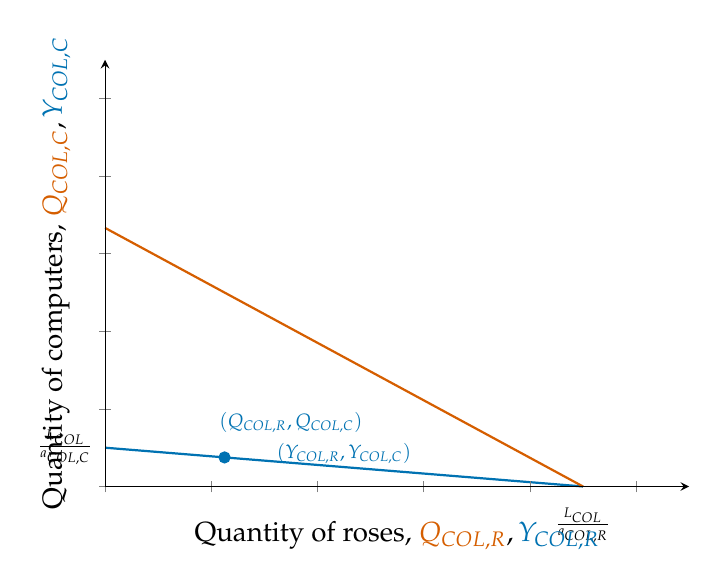
\begin{tikzpicture}
\pgfmathsetmacro{\aC}{900}       % unit labor requirement for computers
\pgfmathsetmacro{\aR}{1}         % unit labor requirement for roses
\pgfmathsetmacro{\alpha}{0.75}    % preference for computers
\pgfmathsetmacro{\Lendow}{9}    % labor endowment

% Compute equilibrium quantities
\pgfmathsetmacro{\Qc}{(\alpha*\Lendow)/\aC}
\pgfmathsetmacro{\Qr}{((1 - \alpha)*\Lendow)/\aR}

% Compute utility level
\pgfmathsetmacro{\U}{(\Qc^(\alpha))*(\Qr^(1 - \alpha))}

% Compute prefactor for indifference curve: Qc = A * Qr^(- (1 - alpha)/alpha)
\pgfmathsetmacro{\expo}{(1 - \alpha)/\alpha}
\pgfmathsetmacro{\A}{\U^(1/\alpha)}

\centering
\begin{axis}[
    ylabel={Quantity of computers, $\textcolor{red}{Q_{COL,C}}, \textcolor{blue}{Y_{COL,C}}$},
    xlabel={Quantity of roses, $\textcolor{red}{Q_{COL,R}}, \textcolor{blue}{Y_{COL,R}}$},
    ymin=0, ymax=0.11,
    xmin=0, xmax=11,
    yticklabel=\empty,
    xticklabel=\empty,
    axis lines=left,
    enlargelimits=false,
    clip=false,
    axis on top,
    scaled x ticks=false,
    width=9cm, height=7cm,
    title style={font=\bfseries}
]

% PPF: Q_C = (L/a_C) - (a_R/a_C) * Q_R
\addplot[thick, blue, domain=0:9] {\Lendow/\aC - (\aR/\aC)*x};

\addplot[thick, red, domain=0:9] {1/15 - (1/135)*x};


% Indifference curve through optimal bundle
%\addplot[red, domain=0.1:9, samples=100] {\A * x^(-\expo)};

% Labels

%\node at (axis cs:3.5,0.03) {\Large $\mathcal{Y}_{US}$};
\node at (axis cs:\Lendow/\aR,-.01) {\scriptsize $\frac{L_{COL}}{a_{COL,R}}$};
\node at (axis cs:-.75,\Lendow/\aC) {\scriptsize $\frac{L_{COL}}{a_{COL,C}}$};


% Equilibrium point
\addplot[only marks, mark=*, color=blue, mark size=2pt] coordinates {(\Qr, \Qc)};
\node at (axis cs:\Qr + 1.25,\Qc + 0.009) {\scriptsize $\textcolor{blue}{(Q_{COL,R},Q_{COL,C})}$};
\node at (axis cs:\Qr + 2.25,\Qc + 0.001) {\scriptsize $\textcolor{blue}{(Y_{COL,R},Y_{COL,C})}$};

\end{axis}

\end{tikzpicture}
}

\end{subfigure}

\caption{Autarky Equilibrium + Trade Prices = More possibilities for Consumption}
\end{figure}
\end{center}
\end{frame}

\section{Epilogue}


\begin{frame}{How is this a ``model''? (deep dive next class)}
    \begin{wideitemize} 
        \item \blue{Parameters and exogenous variables}:
        \begin{itemize}
            \item Endowments (as we will see, number of workers/labor hours)
            \item Technology (as we will see, labor productivity -- i.e., how many hours necessary to produce each good)
        \end{itemize}
        \item<2-> \blue{Model}:
        \begin{itemize}
            \item Firms maximize profits
            \item Consumers maximize utility
            \item Supply = demand
        \end{itemize}
        \item<3-> \blue{Endogenous variables}:
        \begin{itemize}
            \item \textbf{Quantities produced} of each good in each country are optimal for producers
            \item \textbf{Quantities consumed} of each good in each country are optimal for consumers
            \item \textbf{Prices} adjust such that supply = demand
        \end{itemize}
    \end{wideitemize}
\end{frame}



\begin{frame}{The limits to this model (and models in general)}
    \begin{wideitemize} 
        \item Models are useful: they are transparent; conclusion follows logical derivation from premisses
        \item<2-> They are deliberately \textbf{not} reality: abstracts from the unimportant
to focus on a particular mechanism
        \item<3-> But they might be wrong...
        \item<4-> Economics in general requires careful thought about:
        \begin{itemize}
            \item How the model assumptions affect the model outcomes
(``thinking within the model'')
            \item What other aspects are missing from the model that may affect the outcomes in reality (``thinking outside the model'').
\end{itemize}
        \item<5-> E.g.: Americans who worked in industries more exposed to increased competition of imports from China were (relatively) worse off (\href{https://www.aeaweb.org/articles?id=10.1257/aer.103.6.2121}{Autor, Dorn, \& Hanson, 2013})

        \item<6-> Even though the US benefits in aggregate terms (\href{https://onlinelibrary.wiley.com/doi/abs/10.3982/ECTA13758}{Caliendo, Dvorkin, \& Parro, 2019}), there were distributional consequences
    \end{wideitemize}
\end{frame}



\end{document}
